\section{Maximum Torque}
% 
In order to constraint the maximum traction and braking torque one can chose different approaches. This choice depend on the kind of model that describes the dynamic of the motorcycle. In particular, the difference is between the control in torque or in slip.
%
\subsection{Slip}
%
In the slip control a tailored function must be created to compute the torque. In this case we are not making use of the two euler equation of the wheels rotation, therefore those can be solved for the front and the rear torque $\it Myr$ and $\it Myf$. Those are depending on differential terms, however one can simplify the dynamic parts in first approximation and compute the torque only as a function of the states. This mean that one can build a user defined function and limit the torques in the following way.
%
\begin{equation}
    {\it Myf}(\zeta) \ge -{\it Myf_{maxB}}
\end{equation}
%
where ${\it Myf_{maxB}}$ is a positive constant representing the maximum braking torque at the front wheel.
%
\begin{equation}
    {\it Myr}(\zeta) \ge -{\it Myr_{maxB}}
\end{equation}
%
where ${\it Myr_{maxB}}$ is a positive constant representing the maximum braking torque at the rear wheel.
%
\begin{equation}
    {\it Myr}(\zeta) \le {\it MaxTorque}(\omega_r)
\end{equation}
%
where ${\it MaxTorque}(\omega_r)$ is a function of the angular velocity and represent the maximum torque that the ICE can produce. It will be explained in the next sections.
%
\subsection{Torque}
%
When controlling the motorcycle in torque one can restrain the maximum momentum applied at each wheel directly in the dynamic equation. This will be highlighted in section \ref{sec:AddDyn}. The idea is the same as the one of the previous section. The front wheel can brake up to a certain value ${\it Myf_{maxB}}$ as well as the rear (${\it Myr_{maxB}}$).
%
\subsection{MaxTorque}
\label{subsec:MaxT}
%
The ${\it MaxTorque}$ function is a spline roughly derived from empirical data of a racing motorcycle, an Aprilia RSV1000. The data tor torque of the motor at different $\it rpm$ is converted in $\si{\radian/\second}$. Then with the gear ratio data one can retrieve the torque at the wheel as a function of the angular velocity represented in the following graph (Figure \ref{fig:MaxTorque}).\\
%
\begin{figure}[htb]
    \centering
    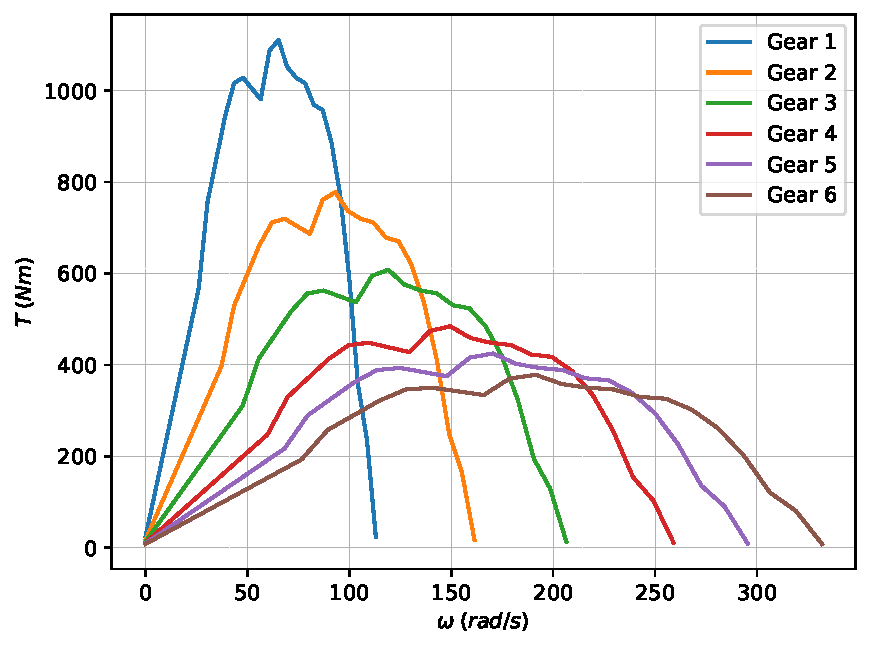
\includegraphics[width=0.9\linewidth]{MaxTorque/maxT_wr.pdf}
    \caption{Maximum torque as a function of angular speed}
    \label{fig:MaxTorque}
\end{figure}
%
The torque data, the $\it rpm$ and the gear ratios are reported in table \ref{tab:TorqueVsRpm} and \ref{tab:GearRatio} in appendix \ref{app:TorqueData}. 



